%------------------------------------------------------
\subsection{Motivation}
%------------------------------------------------------
\begin{frame} %%Eine Folie
  	\frametitle{Motivation}
  	
\end{frame}
%------------------------------------------------------
\begin{frame} %%Eine Folie
  	\frametitle{Motivation}
  	\begin{center}
  	\small Technologieübersicht verschiedener Tracking-Methoden.
  	\end{center}
%
	\begin{table} [H]
		\begin{center}
			\begin{tabular}{rllll}
				\textbf{Arbeitsweise} & \textbf{Optisch} & \textbf{Magnetisch} & \textbf{Ultraschall} & \textbf{ Funk (UHF)} \\
				\textbf{Genauigkeit} & gut & ausreichend & gut & sehr gut \\
				\textbf{Frequenz} & mittel & hoch & gering & hoch \\
				\textbf{Volumen} & mittel & klein & mittel & groß \\
				\textbf{LOS} & Ja & Ja & Nein & Nein \\
				\textbf{In Vivo} & Nein   & Nein & Nein & Ja \\
%			
			\end{tabular}
		\end{center}
		\label{tab:overview_tracking}
	\end{table}  	
\end{frame}
%------------------------------------------------------
\begin{frame} %%Eine Folie
  	\frametitle{Probleme bei Funksystemen}
	\begin{textblock*}{4cm}(8cm,1cm) % {block width} (coords)
		\centering
  		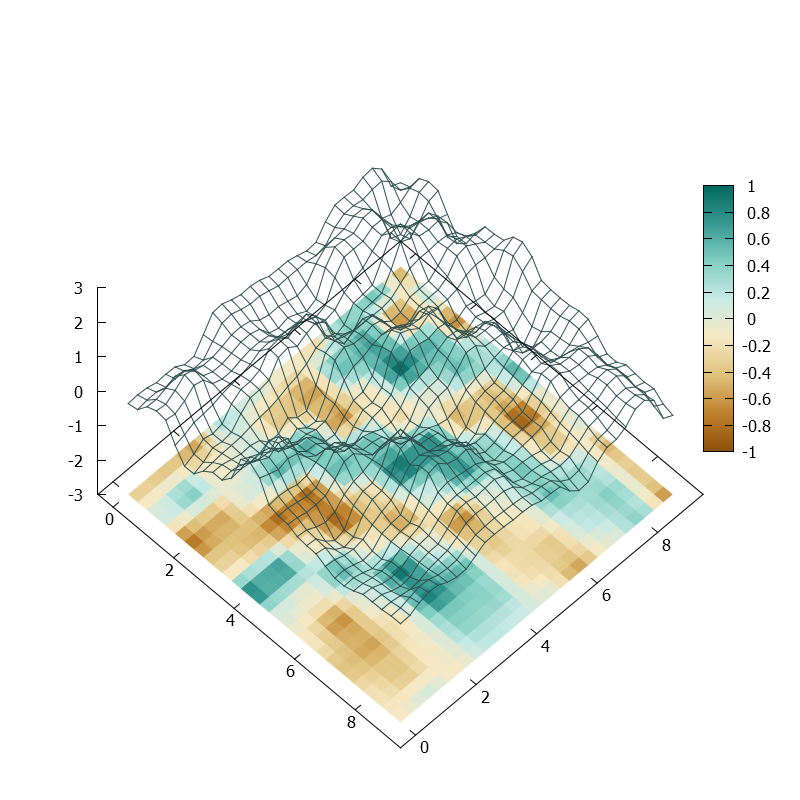
\includegraphics[width=4cm]{../img/Plate0_A1.png}
  	\end{textblock*}
%  	
	\begin{textblock*}{4cm}(8cm,5cm) % {block width} (coords)
		\centering
  		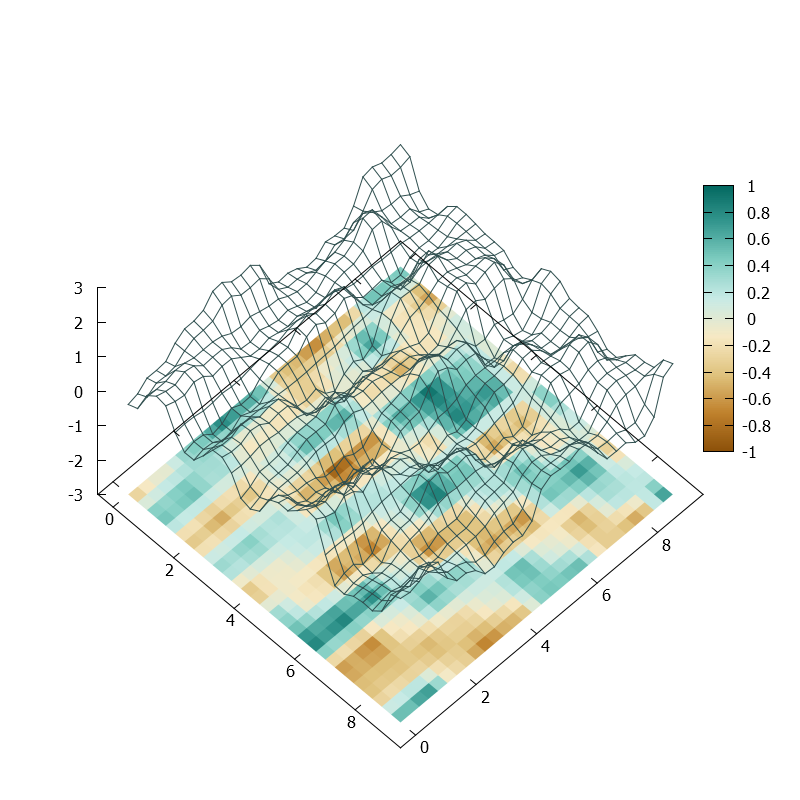
\includegraphics[width=4cm]{../img/Plate0_A4.png}
  	\end{textblock*}
%  	
	\begin{textblock*}{4cm}(2cm,4cm) % {block width} (coords)
  			\begin{itemize}
  				\item Tag Orientierung
  				\item Lesefehler
   				\item Signalauslöschung
   				\item Reflektionen
  		  	\end{itemize}
  	\end{textblock*}
\end{frame}
%------------------------------------------------------
\subsection{System der amedo STS}
\begin{frame}
  \frametitle{Messystem}
	\begin{textblock*}{5cm}(7cm,2cm) % {block width} (coords)
  		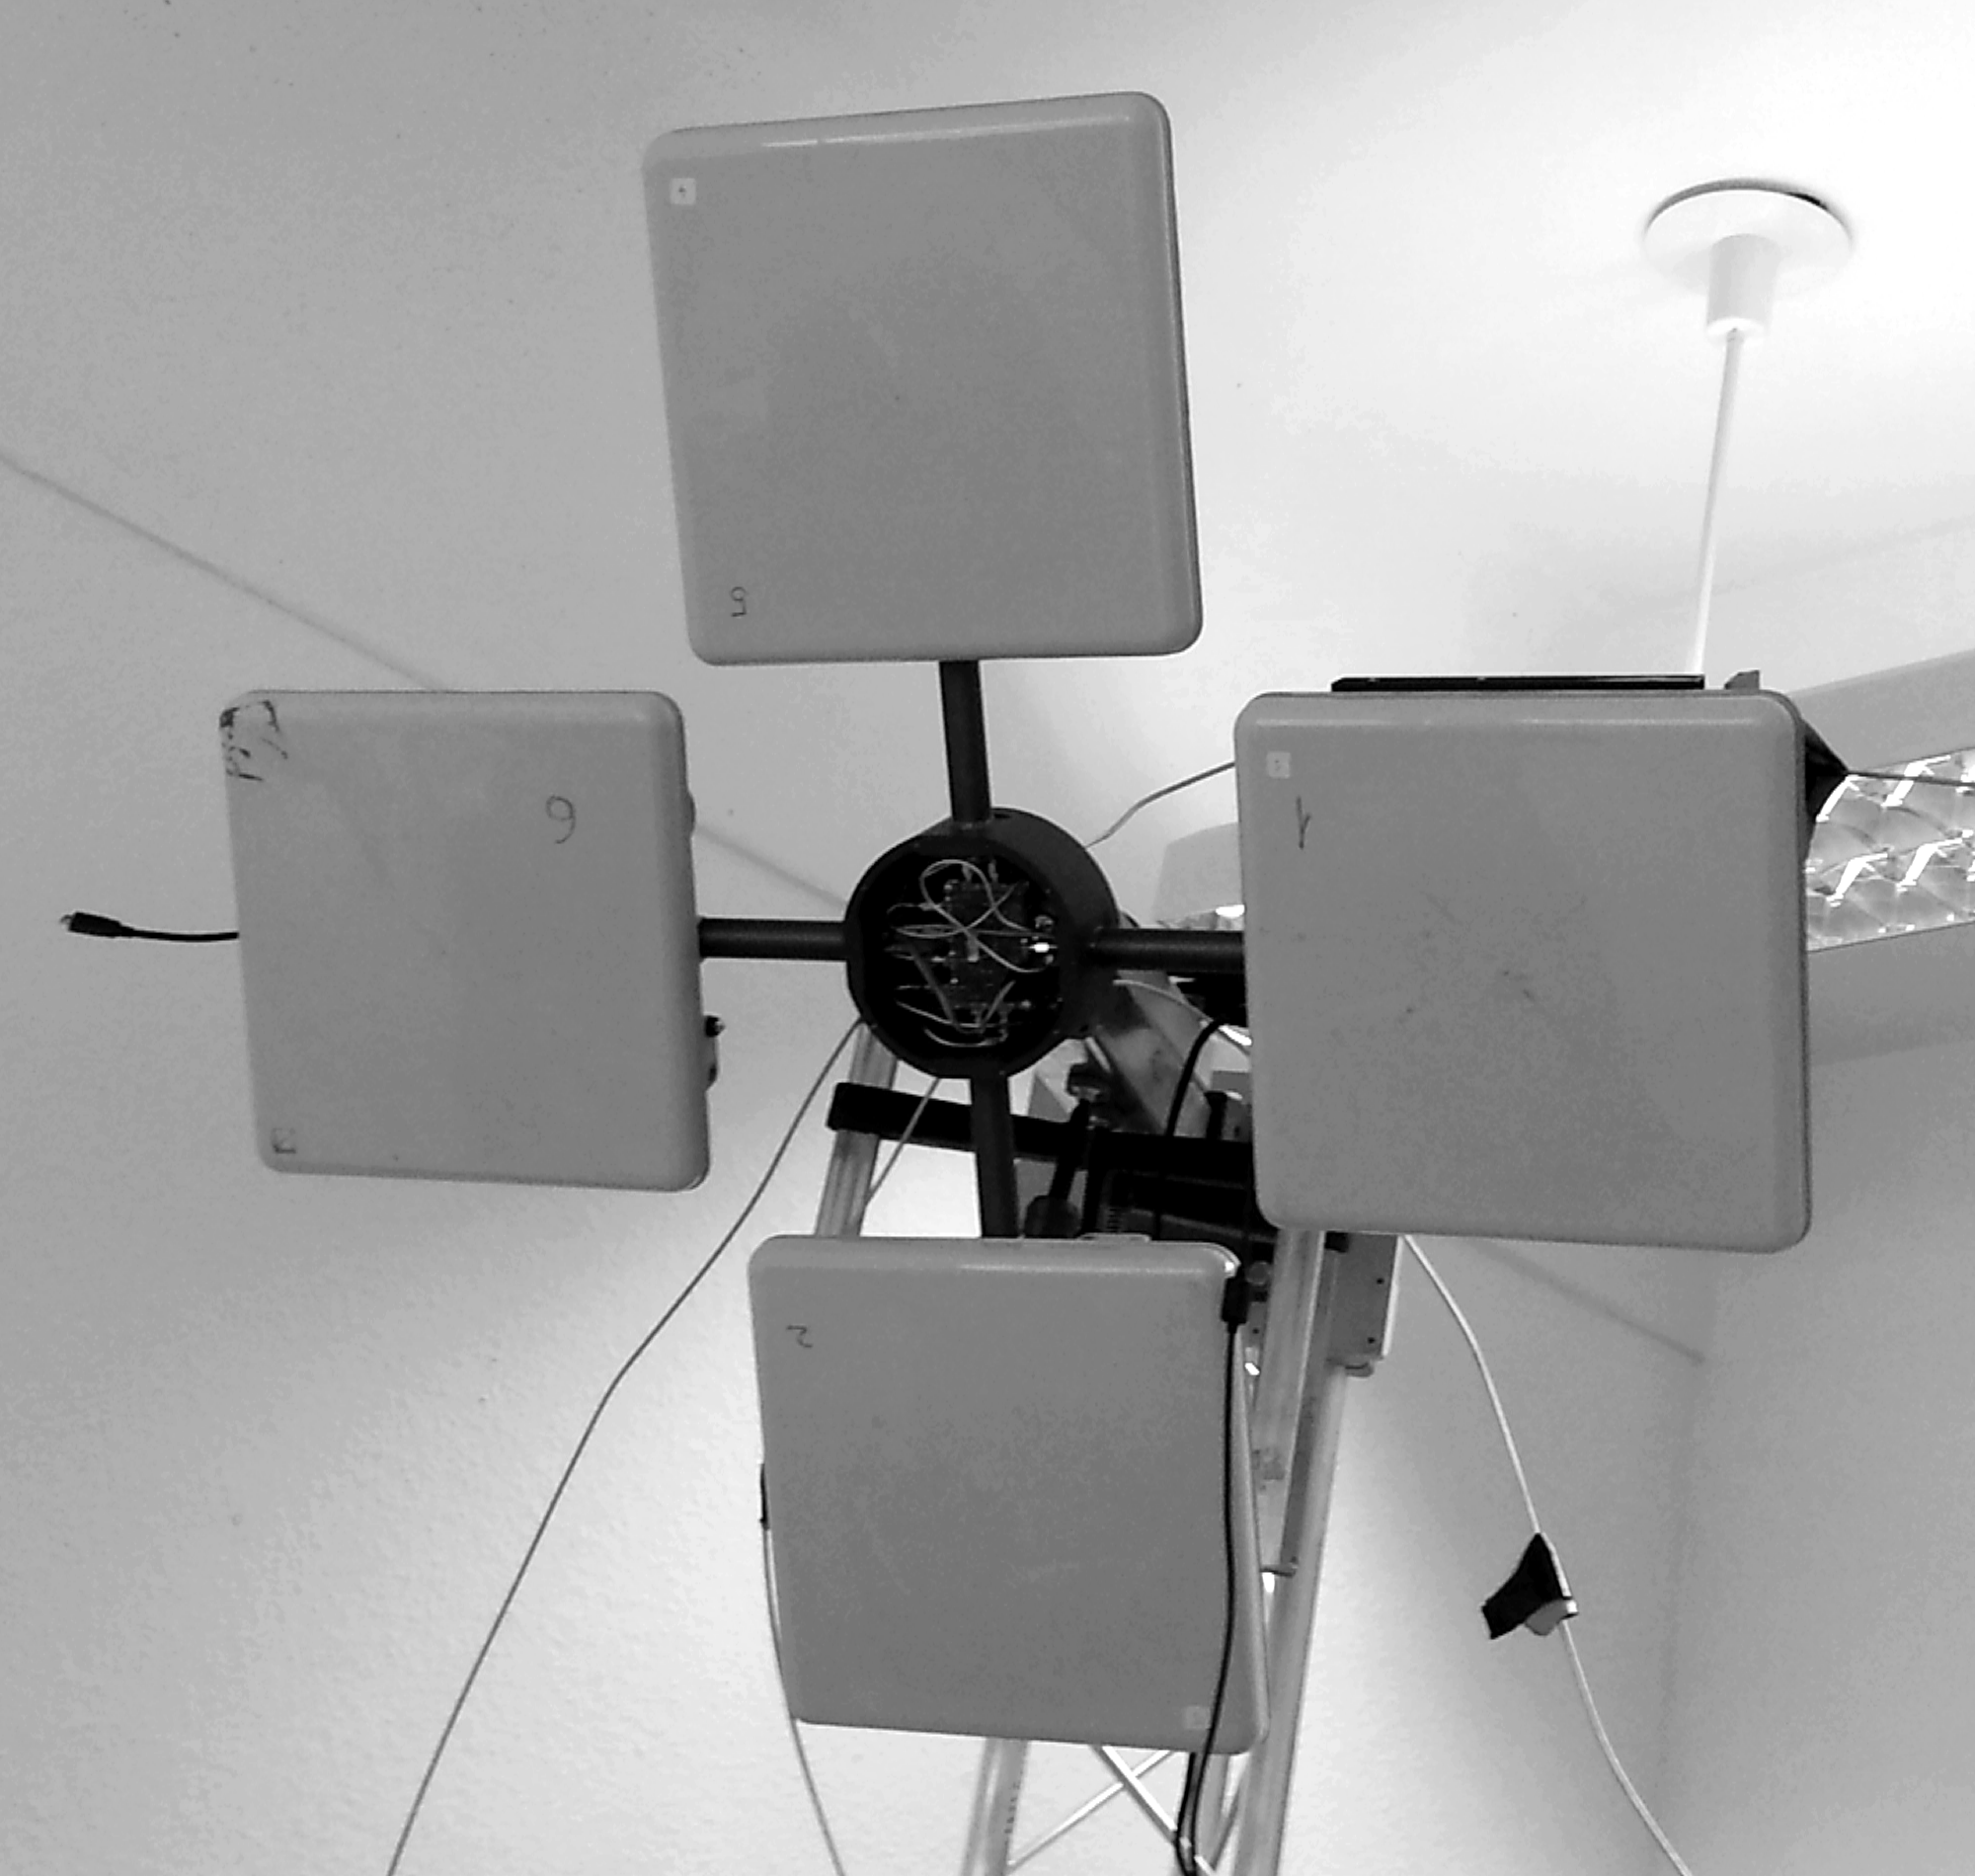
\includegraphics[width=5cm]{../img/4AntennaSetup_small.png}
  	\end{textblock*}
  	\begin{textblock*}{5cm}(.5cm,3cm) % {block width} (coords)
  		\begin{prps}
  		Passive RFID Positioning System
  		\end{prps}
  	\end{textblock*}
\end{frame}
%------------------------------------------------------
\begin{frame}
  \frametitle{Messystem}
	\begin{textblock*}{7cm}(5cm,2cm) % {block width} (coords)
  		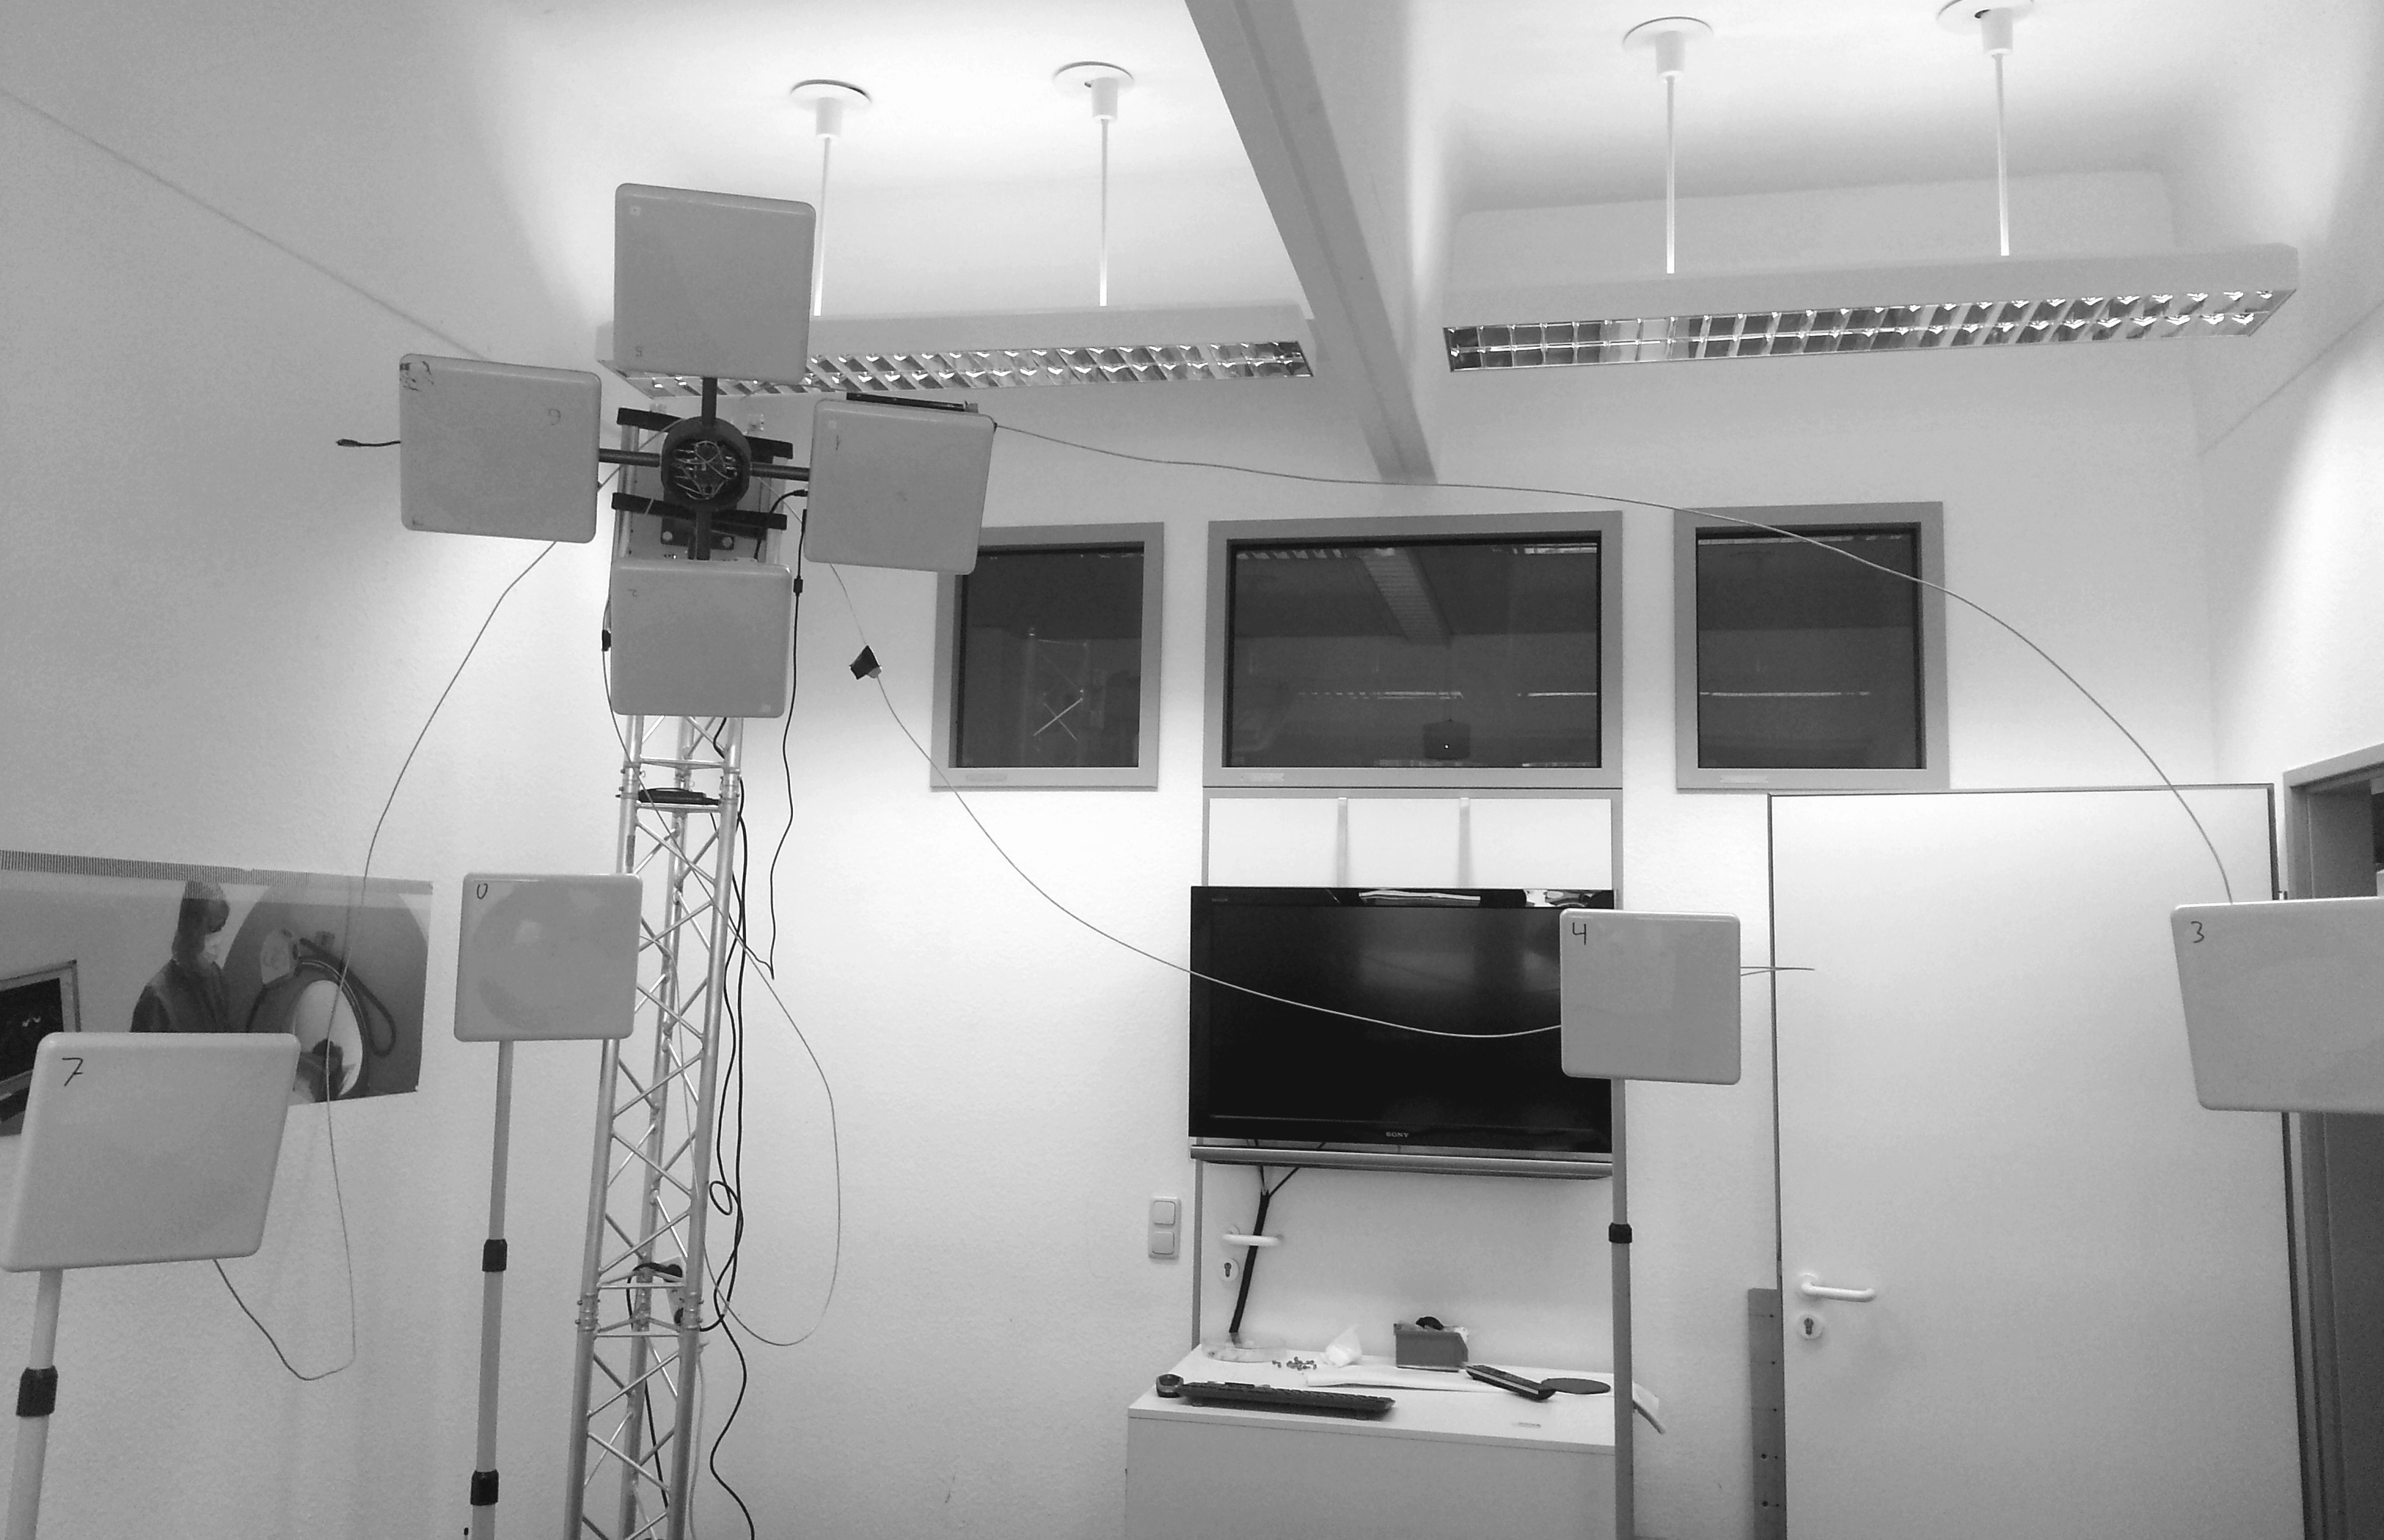
\includegraphics[width=7cm]{../img/RFID-Okto.png}
  	\end{textblock*}
\end{frame}
%------------------------------------------------------
\subsection{Grundlagen}
%------------------------------------------------------
\begin{frame}{Graphics} 
	\frametitle{Mathematische Grundlagen I }
	\centering
	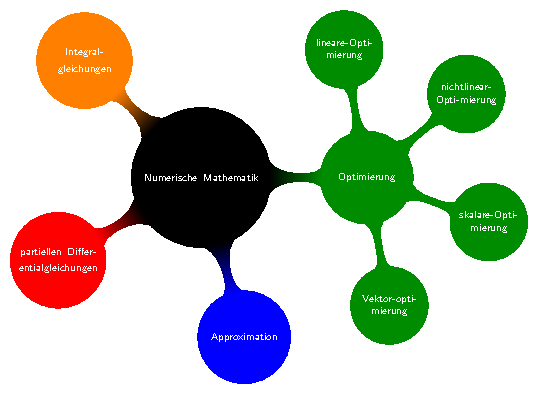
\includegraphics[page=1, width=.6\textwidth]{../img/mindmap.pdf}\\
%--
	\tiny Evolutionäre Verfahren sind Teilgebiet der \textbf{nichtlinearen Optimierung}
\end{frame}
%------------------------------------------------------
\begin{frame}{Graphics} 
  	\frametitle{Mathematische Grundlagen II}
  	\begin{textblock*}{6cm}(6cm,2cm) % {block width} (coords)
   		\includegraphics[page=1, width=6cm]{../img/FlowChart_EvolutionaryOptimization.pdf}
   	\end{textblock*}
%	
	\begin{textblock*}{5cm}(.5cm,3cm) % {block width} (coords)
		\small
   		\begin{ziel}
   		$ y=min\{f(\mathbf{x})\} = -max\{-f(\mathbf{x})\} $
   		\end{ziel}
%   		
		\begin{itemize}
		\item Nichtlineare Optimierung
		\item Ableitungsfrei
		\end{itemize}
   	\end{textblock*}
\end{frame}
%------------------------------------------------------
\begin{frame}{Graphics} 
  	\frametitle{Mathematische Grundlagen III}
%  	
  	\begin{textblock*}{7.5cm}(5cm,2cm) % {block width} (coords)
  		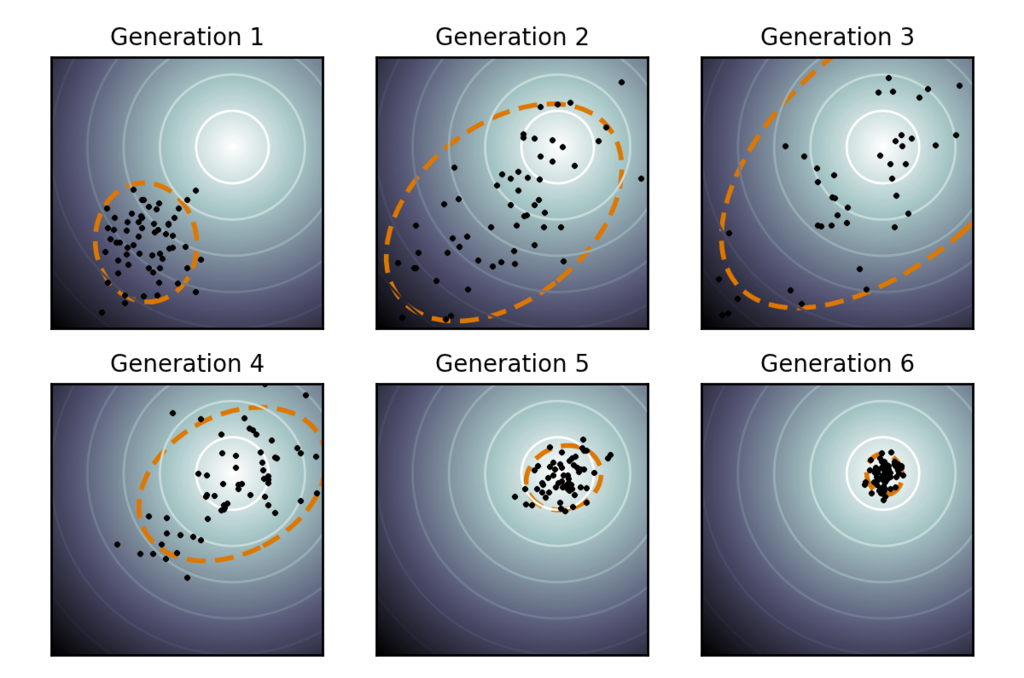
\includegraphics[width=7.5cm]{../img/Concept_of_directional_optimization_in_CMA-ES_algorithm.png}
  		\footnote{Grafik entnommen aus \url{http://en.wikipedia.org/w/index.php?title=File:Concept_of_directional_optimization_in_CMA-ES_algorithm.png&oldid=532567533}}
  	\end{textblock*}
%  	
	\begin{textblock*}{4cm}(.5cm,2.5cm) % {block width} (coords)
		\small
		\begin{cmaes} 
			Covariance Matrix Adaption\\
			$x_{k+1} \sim\ m_k + \sigma_k\times\mathcal{N}(0,C_k)$
		\end{cmaes}
		\small		
  		\begin{itemize}
  	
  		\item Kovarianz Matrix steuert Entwicklung der Population
  		\item Anpassung an die Höhenlinien der Objektfunktion
%  		
  		\end{itemize}
  	\end{textblock*}
%  	
\end{frame}
%------------------------------------------------------
\begin{frame} %%Eine Folie
  \frametitle{Beispiele}
%  
 	\begin{vids}
		Videos zur Veranschaulichung...
 	\end{vids}
%  \begin{itemize}
%	\item\movie[width=1cm,height=1cm,externalviewer]{Video 1}{../vid/vid1.webm}
%	\item\movie[width=1cm,height=1cm,externalviewer]{Video 2}{../vid/vid1.webm}
%	\item\movie[width=1cm,height=1cm,externalviewer]{Video 3}{../vid/vid1.webm}
%	\item\movie[width=1cm,height=1cm,externalviewer]{Video 4}{../vid/vid1.webm}
%  \end{itemize}
%  
\end{frame}

%------------------------------------------------------
%\subsection{Grundlagen2}
%\begin{frame}
%  \frametitle{Test}
%  \begin{fazit} %%Definition
%    Beschreibung des Problems
%  \end{fazit}
%\end{frame}
